\documentclass[a4paper,12pt]{article}

\usepackage[utf8]{inputenc}
\usepackage[T1]{fontenc}
\usepackage{amsmath}
\usepackage{booktabs}
\usepackage{graphicx}
\usepackage{geometry}
\geometry{margin=2.5cm}
\usepackage{xcolor}
\usepackage{listings}
\usepackage{hyperref}
\hypersetup{colorlinks=true, linkcolor=blue!50!black, urlcolor=blue!50!black}
\renewcommand{\tablename}{Tabela}
\renewcommand{\lstlistingname}{Código}

% ---------- Configuração do realce de sintaxe (C) ----------
\definecolor{codebg}{RGB}{247,247,247}
\definecolor{codekw}{RGB}{0,0,180}
\definecolor{codecomment}{RGB}{0,128,0}
\definecolor{codestring}{RGB}{163,21,21}
\definecolor{framecolor}{RGB}{200,200,200}

\lstdefinestyle{cstyle}{
    language=C,
    backgroundcolor=\color{codebg},
    basicstyle=\ttfamily\footnotesize,
    keywordstyle=\color{codekw}\bfseries,
    commentstyle=\color{codecomment}\itshape,
    stringstyle=\color{codestring},
    numberstyle=\tiny\color{gray},
    numbers=left,
    numbersep=6pt,
    frame=single,
    rulecolor=\color{framecolor},
    breaklines=true,
    breakatwhitespace=false,
    showstringspaces=false,
    tabsize=4,
    captionpos=b,
    columns=flexible,
    morekeywords={size_t},
    extendedchars=true,
    literate=
        {á}{{\'a}}1 {à}{{\`a}}1 {â}{{\^a}}1 {ã}{{\~a}}1
        {é}{{\'e}}1 {ê}{{\^e}}1 {í}{{\'i}}1
        {ó}{{\'o}}1 {ô}{{\^o}}1 {õ}{{\~o}}1
        {ú}{{\'u}}1 {ü}{{\"u}}1 {ç}{{\c c}}1
        {Á}{{\'A}}1 {À}{{\`A}}1 {Â}{{\^A}}1 {Ã}{{\~A}}1
        {É}{{\'E}}1 {Ê}{{\^E}}1 {Í}{{\'I}}1
        {Ó}{{\'O}}1 {Ô}{{\^O}}1 {Õ}{{\~O}}1
        {Ú}{{\'U}}1 {Ü}{{\"U}}1 {Ç}{{\c C}}1
}

\title{Tarefa 6: Escopo de Variáveis e Regiões Críticas em OpenMP}
\author{Israel Soares de Castro Filho \\ Matrícula: 20250070780}
\date{}

\begin{document}

\maketitle

\section{Introdução}

Este trabalho tem como objetivo estudar, na prática, os conceitos de escopo de variáveis e regiões críticas em programação paralela com OpenMP, 
usando como estudo de caso a estimativa estocástica do número $\pi$ pelo método de Monte Carlo. A ideia do método é gerar pontos aleatórios uniformemente distribuídos 
no quadrado $[-1,1]\times[-1,1]$ e contar a fração deles que cai dentro do círculo unitário inscrito; como a razão entre as áreas do círculo e do quadrado é $\pi/4$, tem-se

\[
\pi \approx 4 \cdot \frac{n_{\text{dentro}}}{n_{\text{total}}}.
\]

Diferentemente de métodos determinísticos (como a série de Gregory--Leibniz), 
esse problema é interessante para o estudo de paralelismo porque a etapa de contagem envolve uma variável compartilhada 
(\texttt{dentro}) atualizada por todas as iterações, o que expõe de forma direta o problema de \emph{condição de corrida} 
quando o laço é paralelizado ingenuamente. O objetivo específico da tarefa é: 

\begin{enumerate}
    \item Implementar a versão sequencial e uma versão paralela ingênua com \texttt{\#pragma omp parallel for};
    \item Mostrar e explicar o resultado incorreto produzido pela condição de corrida;
    \item Corrigir o problema com \texttt{\#pragma omp critical};
    \item Reestruturar o código separando \texttt{\#pragma omp parallel} e \texttt{\#pragma omp for}, aplicando as cláusulas \texttt{private}, \texttt{firstprivate}, \texttt{lastprivate} e \texttt{shared};
    \item Discutir o papel de \texttt{default(none)} na clareza do escopo em programas complexos.
\end{enumerate}

\section{Metodologia}

O código foi implementado em C (arquivo \texttt{tarefa6.c}, Apêndice~\ref{ap:codigo}) e paralelizado com OpenMP. Foram implementadas quatro versões da estimativa de $\pi$, todas utilizando o mesmo gerador de números pseudoaleatórios \emph{thread-safe} (Xorshift32, com estado passado por referência e nunca inicializado em zero, para evitar a degeneração conhecida desse gerador):

\begin{itemize}
    \item \textbf{Ingênua} (\texttt{pi\_paralelo\_com\_erro}): paraleliza o laço com \texttt{\#pragma omp parallel for} simples, incrementando diretamente uma variável \texttt{long dentro} compartilhada e chamando \texttt{rand()} (função com estado global, não \emph{thread-safe}) dentro da região paralela. Serve para evidenciar a condição de corrida.
    \item \textbf{Critical} (\texttt{pi\_paralelo\_critical}): reestruturada com \texttt{\#pragma omp parallel} seguido de \texttt{\#pragma omp for}, com a semente de cada thread inicializada uma única vez (\texttt{private} implícita por ser declarada dentro do bloco paralelo) e o incremento de \texttt{dentro} protegido por \texttt{\#pragma omp critical} a cada ponto dentro do círculo.
    \item \textbf{Otimizada} (\texttt{pi\_paralelo\_otimizado}): cada thread acumula em um contador local \texttt{dentro\_local} (privado) durante todo o laço \texttt{\#pragma omp for} e só executa uma seção crítica \emph{uma vez}, ao final, para somar seu resultado parcial na variável compartilhada \texttt{dentro\_total}.
    \item \textbf{Reduction} (\texttt{pi\_paralelo\_reduction}): usa a cláusula \texttt{reduction(+:dentro)} no próprio \texttt{\#pragma omp parallel}, deixando o runtime OpenMP responsável por criar cópias privadas por thread e combiná-las automaticamente ao final da região.
\end{itemize}

Além disso, a função \texttt{demonstrar\_clausulas} isola, em um laço simples e independente do problema de Monte Carlo, o efeito de cada cláusula de escopo (\texttt{private}, \texttt{firstprivate}, \texttt{lastprivate}, \texttt{shared}) sobre quatro variáveis de controle (\texttt{a}, \texttt{b}, \texttt{c}, \texttt{d}), permitindo observar diretamente o valor de cada uma antes e depois da região paralela.

Todas as regiões paralelas usam \texttt{default(none)}, exigindo que cada variável usada seja classificada explicitamente. 
A medição de tempo é feita com \texttt{omp\_get\_wtime()} (tempo de relógio, \emph{wall-clock}).

O programa foi compilado com:
\begin{verbatim}
$ gcc -std=c11 -fopenmp -O2 -Wall -o tarefa6 tarefa6.c -lm
\end{verbatim}
e executado em uma máquina com \texttt{omp\_get\_max\_threads() = 20}, testando amostras de $10^3$ a $10^7$ pontos.

\section{Resultados}

A demonstração das cláusulas de escopo produziu a seguinte saída:

\begin{verbatim}
Antes do laco:  a=10  b=10  c=10  d=0
Depois do laco: a=10 (indefinido/nao usar)
                b=10 (inalterado fora, era firstprivate)
                c=7  (deve ser 7, ultima iteracao)
                d=8  (deve ser 8, soma protegida)
\end{verbatim}

Quanto à estimativa de $\pi$ ($\pi_{\text{real}} = 3{,}1415926536$), a versão ingênua produziu valores cada vez mais distantes do correto à medida que o número de pontos cresce: $2{,}956$ ($10^3$ pontos), $0{,}878$ ($10^4$), $0{,}840$ ($10^5$), $0{,}368$ ($10^6$) e $0{,}263$ ($10^7$). Já as versões \emph{Critical}, \emph{Otimizada} e \emph{Reduction} produziram, em cada tamanho de amostra, exatamente o mesmo valor entre si — $3{,}156$; $3{,}1448$; $3{,}14704$; $3{,}138704$; e $3{,}1408096$, respectivamente — todos com erro absoluto decrescente e da ordem de $10^{-3}$ já a partir de $10^6$ pontos, como esperado de uma implementação correta.

A Figura~\ref{fig:tempo} apresenta o tempo de execução de cada versão em função do número de pontos, em escala log-log. Para $10^3$ e $10^4$ pontos, o tempo medido ficou em $0,000\,\text{s}$ para praticamente todas as versões (a exceção foi um único registro de $0{,}001\,\text{s}$ em \emph{Reduction} com $10^3$ pontos, atribuível a ruído de inicialização) — ou seja, abaixo da resolução útil do cronômetro nessas amostras pequenas, sem informação de desempenho a extrair. Por isso, a figura mostra apenas $n = 10^5, 10^6, 10^7$, faixa em que as diferenças entre versões já são mensuráveis; os dois pontos de \emph{Reduction} iguais a zero nessa faixa ($10^5$ e $10^6$) foram marcados com um ``$\times$'' e posicionados em um piso visual, apenas para não quebrar a escala logarítmica.

\begin{figure}[h]
\centering
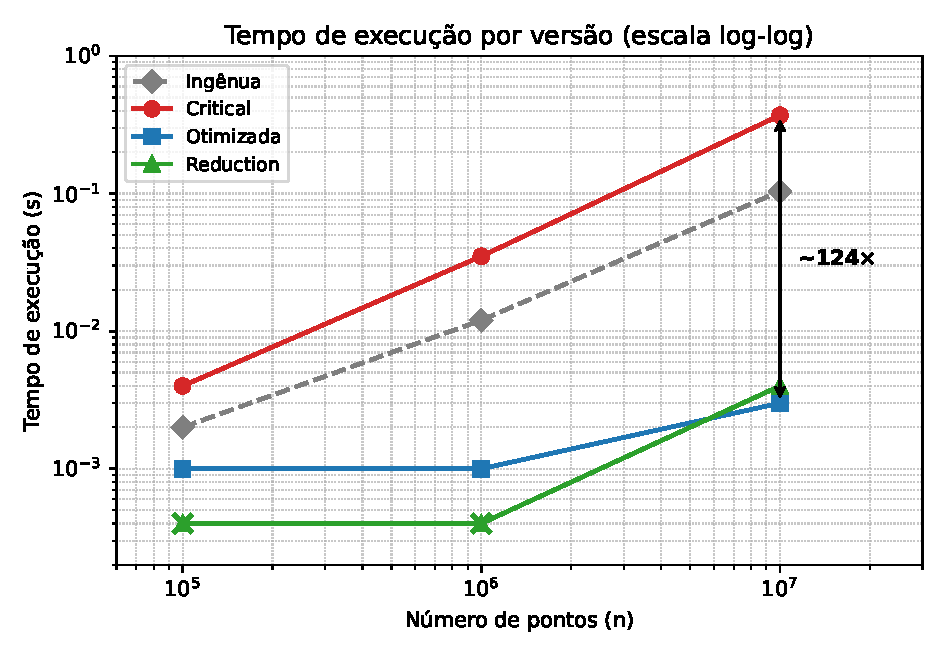
\includegraphics[width=0.85\textwidth]{images/tempo_execucao.pdf}
\caption{Tempo de execução por versão em função do número de pontos (escala log-log). Marcadores ``$\times$'' indicam tempo medido igual a $0,000\,\text{s}$ (abaixo da resolução do cronômetro), reposicionados em um piso visual apenas para permitir a escala log.}
\label{fig:tempo}
\end{figure}

\section{Análise}

\paragraph{O resultado incorreto da versão ingênua.} Os valores de $\pi$ apresentados acima mostram que a versão ingênua não apenas erra, como o erro \emph{cresce sistematicamente} com o número de pontos, em vez de apenas oscilar em torno de $\pi$ como seria esperado de um simples ruído estatístico: o valor estimado cai de $2{,}956$ (com $10^3$ pontos) até $0{,}263$ (com $10^7$ pontos). Isso tem duas causas combinadas:

\begin{enumerate}
    \item \textbf{Condição de corrida em \texttt{dentro++}.} A operação é, na verdade, três passos (ler, incrementar, escrever) que não são atômicos. Com 20 threads disputando a mesma variável, várias leituras ocorrem antes de qualquer escrita ser propagada, de modo que incrementos são perdidos. Quanto mais pontos e mais threads simultâneas, maior a frequência de colisões, então a fração de incrementos perdidos tende a aumentar com $n$ — o que explica o viés crescente observado, e não apenas uma dispersão aleatória em torno do valor correto.
    \item \textbf{\texttt{rand()} não é \emph{thread-safe}.} A função mantém estado interno global; chamadas concorrentes de 20 threads corrompem esse estado, de modo que os valores gerados deixam de ser uma amostra i.i.d.\ válida, o que também contribui para o viés sistemático, e não apenas a perda de incrementos.
\end{enumerate}

\paragraph{Correção com \texttt{critical}.} Ao proteger \texttt{dentro++} com \texttt{\#pragma omp critical} 
e usar um gerador próprio por thread (Xorshift32 com semente independente), o resultado passa a convergir corretamente para 
$\pi$ (erro da ordem de $10^{-3}$ já em $10^6$--$10^7$ pontos). O custo, porém, é alto: como cerca de 78\% dos pontos caem dentro do círculo, 
quase toda iteração do laço precisa entrar na seção crítica, serializando essa fração do trabalho. 
Isso é visível na Figura~\ref{fig:tempo}: em $10^7$ pontos, a versão \emph{Critical} leva $0{,}371$\,s, cerca de \textbf{124 vezes mais lenta} que a versão \emph{Otimizada} ($0{,}003$\,s).

\paragraph{Reestruturação com \texttt{parallel} + \texttt{for} e as cláusulas de escopo.} As versões \emph{Otimizada} e \emph{Reduction} evitam o gargalo movendo a seção crítica para \emph{fora} do laço: cada thread acumula em uma variável local (privada, por ser declarada dentro do bloco \texttt{\#pragma omp parallel}) e só sincroniza uma vez, ao final. O resultado nos tempos é dramático: ambas ficam na faixa de milissegundos mesmo em $10^7$ pontos, contra centenas de milissegundos da versão \emph{Critical}. A saída de \texttt{demonstrar\_clausulas} confirma o comportamento esperado de cada cláusula:

\begin{itemize}
    \item \texttt{private(a)}: cada thread recebe uma cópia isolada de \texttt{a}; como o valor não é propagado de volta, \texttt{a} permanece com o valor anterior à região paralela (10) fora do laço, mesmo tendo sido reescrito internamente.
    \item \texttt{firstprivate(b)}: como \texttt{private}, mas a cópia de cada thread é inicializada com o valor de \texttt{b} anterior ao laço (10); o valor externo também permanece inalterado após a região, pois não há cópia de volta.
    \item \texttt{lastprivate(c)}: ao final da região, \texttt{c} recebe o valor calculado pela iteração sequencialmente \emph{última} do laço ($i=7$), o que foi confirmado pela saída (\texttt{c=7}).
    \item \texttt{shared(d)}: todas as threads acessam a mesma posição de memória; sem proteção (aqui, \texttt{\#pragma omp atomic}), o incremento estaria sujeito à mesma condição de corrida da versão ingênua. Com a proteção, o resultado final foi o esperado (\texttt{d=8}, uma unidade por iteração).
\end{itemize}

\paragraph{Papel de \texttt{default(none)}.} Sem essa cláusula, qualquer variável referenciada dentro de uma região paralela e não classificada explicitamente assume 
por padrão o escopo \texttt{shared} — que foi exatamente a causa raiz do bug da versão ingênua. Com \texttt{default(none)}, o compilador passa a exigir que \emph{toda} 
variável usada na região seja explicitamente declarada como \texttt{private}, \texttt{firstprivate}, \texttt{lastprivate} ou \texttt{shared}; se alguma for esquecida, o código sequer compila.

\section{Conclusão}

O experimento evidenciou de forma concreta como a ausência de controle de escopo em OpenMP leva a condições de corrida com impacto crescente sobre a 
precisão do resultado, e não apenas a ruído aleatório. A correção ingênua com \texttt{\#pragma omp critical} 
resolve a corretude, mas ao custo de um gargalo de sincronização que pode tornar o código paralelo mais lento que o sequencial quando a seção crítica é executada com muita frequência. 

A reestruturação com acumuladores privados por thread (seja manualmente, com \texttt{private} e uma única seção crítica de junção, seja de forma idiomática, 
com \texttt{reduction}) elimina esse gargalo e recupera o ganho de desempenho esperado do paralelismo. 

Por fim, as cláusulas \texttt{private}, \texttt{firstprivate}, \texttt{lastprivate} e \texttt{shared} definem precisamente o que cada thread vê e o que é propagado de volta ao término da região, e \texttt{default(none)} 
torna essas decisões explícitas e verificáveis em tempo de compilação — uma prática recomendável especialmente à medida que o programa cresce em complexidade.

\newpage
\appendix

\section{Código-Fonte}
\label{ap:codigo}

\lstinputlisting[style=cstyle, caption={Código-fonte completo (\texttt{tarefa6.c})}]{../src/tarefa6.c}

\end{document}